\documentclass[12pt,a4paper]{article}
\usepackage[utf8]{inputenc}
\usepackage{graphicx}
\graphicspath{{../Images/}}
\usepackage{amsmath}
\usepackage{multirow}
\usepackage{amsfonts}
\usepackage{amssymb}
\usepackage{hyperref}
\usepackage[margin=1in]{geometry}
\usepackage{ulem}
\usepackage{subfig}
\usepackage{float}
\usepackage{xcolor}
\hypersetup{
    linktoc=all,     %set to all if you want both sections and subsections linked
    linkcolor=blue,  %choose some color if you want links to stand out
}
\usepackage{listings}
\definecolor{dkgreen}{rgb}{0,0.6,0}
\definecolor{gray}{rgb}{0.5,0.5,0.5}
\definecolor{mauve}{rgb}{0.58,0,0.82}

\lstset{frame=tb,
  backgroundcolor=\color[rgb]{0.9,0.9,0.9},
  language=C++,
  aboveskip=3mm,
  belowskip=3mm,
  showstringspaces=false,
  columns=flexible,
  basicstyle={\small\ttfamily},
  numbers=none,
  numberstyle=\tiny\color{gray},
  keywordstyle=\color{blue},
  commentstyle=\color{dkgreen},
  stringstyle=\color{mauve},
  breaklines=true,
  breakatwhitespace=true,
  tabsize=3
  }

\author{Thibaut Marmey}

\title{Notes de cours C++}
\begin{document}
	\maketitle

\begin{normalsize}
\tableofcontents
\end{normalsize}

\section{Formation C++ - Décembre 2018}
\subsection{Généralités}
\subsubsection{L'analyse autour d'un projet}
\begin{itemize}
\item Concevoir c'est créer un système EVOLUTIF + ROBUSTE
\begin{itemize}
\item Maintenance (code à modifier)
\item Robustesse (déterministe, si problème on trouve facilement, gestion des exception...)
\end{itemize}
\item \textbf{La conception est beaucoup plus importante que le developpement}
\item Avant le code, grosse partie d'analyse pour : 
\begin{itemize}
\item comprendre le système
\item concevoir le cahier des charges
\item analyser les relations entre les différents éléments du projets
\end{itemize}
\end{itemize}
\subsubsection{Le concept orienté objet}
\begin{itemize}
\item En orienté objet : \textbf{Le passé a une influence sur le futur}
\item \textit{Main()} est le client
\begin{itemize}
\item Il ne doit y voir que des actions (via les méthodes des classes)
\item C'est un test, un cas réel
\item Il ne devrait donc pas y avoir de if, for etc
\end{itemize}
\item Les classes et les méthodes crées sont les services
\item Conception de base : \textbf{TDR (Test Driven Requirement)}
\begin{itemize}
\item On part de ce que l'on veut \textit{main()}
\item\textbf{couverture fonctionnelle} : on crée juste les méthodes pour compiler le \textit{main()}
\item On implémente les méthodes dans la classe
\end{itemize}
\item En C++ on est proche des objets réels, leur conception se fait en les conceptualisant
\item \textbf{Encapsulation} : dans une même objet il y a des données et des fonctions qui peuvent ne pas être accessible depuis l'extérieur.
\end{itemize}
\subsubsection{Smell-Code vs Clean-Code}
\begin{itemize}
\item Ne pas faire de \textbf{Smell Code}
\begin{itemize}
\item Duplication
\item Appel méthodes d'autres classes
\item BLOB : classe trop importante par rapport aux autres
\item Surnombre d'arguments
\end{itemize}
\item \textbf{La contrainte amène la qualité}
\item \textbf{Clean Code} (qualité logicielle) :
\begin{itemize}
\item méthode courte
\item nom clair
\item économie des messages (méthodes)
\end{itemize}
\item Si méthode trop longue on extrait des lignes de codes pour créer une nouvelle fonction et ensuite placer ces nouvelles méthodes en "private" car ces méthodes ne sont pas utilisé par l'utilisateur !
\item La documentation doit être automatisé par un logiciel : les mises à jour se font au fur et à mesure de l'avancement du code (la doc ne devrait pas être une activité humaine)
\end{itemize}
\subsubsection{Représentation UML}
\begin{itemize}
\item Représenter les choses dont on a besoin : \textbf{UML}
\begin{itemize}
\item Toutes les relations entre les classes "All" (pour celui qui développe le système)
\item Seulement avec les choses "Public" (pour celui qui utilise)
\item Il y a toujours un seul \textit{"system"}, c'est celui qui englobe tout le reste
\end{itemize}
\end{itemize}
\subsubsection{Visual Studio}
\begin{itemize}
\item Documentation CodeOrganization : permet de connaître, visualiser les dépendances entre les différents fichiers
\item Raccourci Visual Studio
\begin{lstlisting}
// ctrl + k -> ctrl + c (comment)
// ctrl + k -> ctrl + u (uncomment)
\end{lstlisting}
\end{itemize}

\subsection{Première Partie}
\subsubsection{Initialisation uniforme et argc/argv, énumération typée}
\begin{itemize}
\item \textbf{C++11} - Initialisation uniforme, donne la valeur par défaut avec les accolades, peut importe le type donné
\begin{lstlisting}
int i {};
float f{};
char c{};
class A a{};

// Dans boucle for
for(int index{};...)
\end{lstlisting}
\item La portée des variables est limitée dans le bloc
\item Dans la fonction \textit{main()}, \textit{argc} est toujours supérieur ou égal à 1 car le premier argument est nécessairement le nom de l'application avec son chemin global.
\begin{lstlisting}
int main(int argc, char** argv){
// argc = arg count >= 1
// argv = arg values
}
\end{lstlisting}
\item Enumeration fortement typée
\begin{lstlisting}
enum class A { }
// Avant on ne pouvait pas avoir deux enum COLOR{VERT, blabla} et ETAT{VERT, blabla}. Il y avait un conflit entre les deux variables "VERT".
\end{lstlisting}
\end{itemize}
\subsubsection{Boucle For-Each \& Do-While}
\begin{itemize}
\item La boucle FOR EACH
\begin{lstlisting}
for (int n : tab) { }  // Par recopie
for (int& n : tab) { } // Par reference (on modifie directement les elements)
Dice tab[10] // Tableau de 10 objets Dice
for (Dice& d : tab) // Parcour de tab par reference
\end{lstlisting}
\item La boucle DO-WHILE (passe au moins une fois dans la boucle, contrairement au \textit{while} simple)
\begin{lstlisting}
do{ blabla bla } while(condition)
\end{lstlisting}
\end{itemize}
\subsubsection{Array}
\begin{itemize}
\item Pour un tableau de taille fixe utiliser \textit{array}
\begin{lstlisting}
array<type, size> name{values...}
\end{lstlisting}
\end{itemize}
\subsubsection{Liste d'initialisation générique}
\begin{itemize}
\item Listes d'initialisation génériques : fonctions à paramètres variables
\begin{lstlisting}
#include <initialiser_list>

int somme (initializer_list<type> liste) {
// bla bla
}
// Dans main(), appel de la fonction
somme( {a,b,c,d} );
\end{lstlisting}
\end{itemize}

\subsection{Deuxième Partie}
\subsubsection{Using \& this}
\begin{itemize}
\item \textbf{C++11} - utiliser USING pour créer un nouveau nom de type de variable
\begin{lstlisting}
using Vitesse = int;
\end{lstlisting}
\item Utilisation de \textit{this} si conflit entre méthode de la fonction et attribut de la classe
\begin{lstlisting}
// Dans methode changerAltitude(int altitude)
this->altitude = altitude;
// this->altitude : pointeur sur l'objet de la classe
// altitude : argument de la fonction
\end{lstlisting}
\end{itemize}
\subsubsection{La ZIM}
\begin{itemize}
\item Toujours initialiser les membres de la classe dans la \textbf{ZIM} : \textbf{zone d'initialisation des membres}.
\begin{lstlisting}
//Constructeur de la classe nomClasse
public:
	nomClasse() : --ZIM-- {};
\end{lstlisting}
\item Les constructeurs n'ont pas de type de fonction car ce n'est pas nous qui les appelons
\end{itemize}
\subsubsection{Self-delegation}
\begin{itemize}
\item \textbf{Self-delegation} : la classe s'envoie un message à elle toute seule (permet d'éviter le smell code)\\
Exemple : dans la classe Dice, on initialise la faceValue par la méthode roll().
\end{itemize}
\subsubsection{Rand \& srand}
\begin{itemize}
\item RAND \& SRAND pour créer des séquences aléatoires. Il faut utiliser \textit{srand} pour réarmer le \textit{seed} de \textit{rand}
\begin{lstlisting}
#include <ctime>
srand(time(nullptr)); // Ne pas mettre dans le main
\end{lstlisting}
\end{itemize}
\subsubsection{Méthode setup}
\begin{itemize}
\item ".setup" : pour modifier l'objet qui a été créé. C'est une méthode très utilisée (ex interfaces graphiques ou jeu démineur).\\
Le jeu (objet) est d'abord créé puis on modifie sa configuration (beginner, expert,...) et on actualise le jeu via la méthode de l'objet jeu ".setup".
\end{itemize}

\subsection{Troisième Partie}
\subsubsection{Organisation du code}
\begin{itemize}
\item Importation des fichiers systèmes (librairies standard C++) avec les chevrons
\item Importation des fichiers locaux (les .h) avec les guillemets
\item Pour les commandes du pré-processeur on n'utilise pas le point virgule
\item Création de fichiers d'en tête : les fichiers ".h"
\begin{itemize}
\item On stipule que le fichier doit être inclu qu'une seule fois
\begin{lstlisting}
#pragma once
\end{lstlisting}
\end{itemize}
\item Le pré-processeur fait la concaténation des fichiers avec le \textit{\#include}.
\item \#define est utilisé en C mais il faut arréter en C++.
\item Séparer le contrat ".h" de l'implémentation ".cpp".
\begin{itemize}
\item \textbf{Le contrat} : décrit les fonctions mais pas de code (dit ce dont tu as besoin en entrée)
\item \textbf{l'implémentation} : décrit le code des méthodes
\end{itemize}
\item Opérateur de résolution de portée "\textbf{::}"
\item \textbf{Bonne pratique} : créer le fichier "util.h" pour inclure des librairies toujours utilisées, des \textit{"using std::"}, ou le petit matériel comme les \textit{"using"}. L'inclure dans le grain de classe le plus faible.
\begin{lstlisting}
#include <string>
using std::string
\end{lstlisting}
\item Ne pas inclure de \textit{using namespace} dans un contrat (.h) car on donne l'accès à beaucoup trop de choses et donc risque de collision, etc... On utilisera donc l'opérateur de résolution de portée dans les .h\\
On peut donc inclure les \textit{using namespace} dans les .cpp
\subsubsection{Inline}
\item Fonction/Méthode \textbf{inline}, c'est une fonction implémentée directement dans le contrat ".h". Ce sont des méthodes accesseures de data, celle qui retourne directement une data.
\begin{lstlisting}
// Dans le .h
inline int getData() {return data}

// On ne fait pas de methode inline si la valeur retournee est une fonction mathematique complexe
\end{lstlisting}
\subsubsection{La constance}
\item La \textbf{constance} : si on sait que la fonction ne doit pas avoir d'effet de bord on utilise \textit{const}
\begin{lstlisting}
type nomMethode(...) const {bla bla}
\end{lstlisting}
La constance est différente du const pour les variables.
\end{itemize}

\subsection{Quatrième Partie}
\subsubsection{Données et méthodes statiques}
\begin{itemize}
\item Les données et méthodes statiques : ce sont des éléments partagés par toutes les instances de la classe. Ce sont des données de classe, on utilise \textit{static inline} pour les déclarer.
\begin{lstlisting}
static inline type nomData; // C++17
\end{lstlisting}
\item Ex avec la classe Voiture :
\begin{itemize}
\item attribut de classe : la vitesse max sur les routes en France
\item attribut d'objet : la couleur d'une voiture
\end{itemize}
\item \textit{Static} n'a rien à voir avec "ne bouge pas". Ça veut dire que ça appartient à la classe.
\item Une méthode statique peut seulement accéder aux attributs statiques
\begin{lstlisting}
static nomMethode() {return data} // Avec data un membre "static inline"
\end{lstlisting}
\item Utilisation dans le \textit{main()} (c'est un message envoyé à la classe et non à une instance de classe)
\begin{lstlisting}
nomClasse::nomMethodeStatique();
\end{lstlisting}
\item On ne peut donc pas utilisé de \textit{this} dans un méthode statique
\item Exemple d'utilisation : connaitre le nombre d'instances existants d'une classe
\begin{itemize}
\item utiliser attribut de classe
\item Incrémenter dans le constructeur
\item décrémenter dans le destructeur
\item Récupérer attribut de classe via une méthode de classe (une méthode statique)
\end{itemize}
\item \textbf{C++11} - On ne peut pas initialiser la variable statique directement dans le .h. Il faut passer par le .cpp
\begin{lstlisting}
type nomClasse::varStatique{value}
\end{lstlisting}
\item Dans la méthode statiques utiliser les "\textbf{::}" pour modifier l'attribut statique
\end{itemize}

\subsection{Cinquième Partie}
\subsubsection{Gestion des excpetions}
\begin{itemize}
\item Phase de développement \\\\
\begin{tabular}{|c|c|c|}
  \hline
  1-Maquette & 2-Prototype & 3-Livrable \\ \hline
  pas de code & code nominal & rajouter les cas d'erreurs\\\hline
\end{tabular}
\item \textbf{Programmation défensive} : la faute de programmation est différente de la faute de l'utilisateur (situation métier qui doit être pris en compte)
\item \textbf{Faute de programmation} : pour corriger un bug de conception on utilise des \textbf{ASSERT}.
\begin{itemize}
\item On peut mettre des assert de partout, ensuite régler les problèmes
\item Utiliser \textit{NDEBUG} pour ne plus exécuter les assertions
\begin{lstlisting}
#include <cassert>
// #define NDEBUG
assert(condition)
\end{lstlisting}
\end{itemize}
\item \textbf{Faute de l'utilisateur} : pour gérer les \textbf{exception} \textbf{(pur C++)}
\begin{lstlisting}
// Dans util.h
#include <exception>
using std::exception

// Dans methode
throw exception

// Dans main()
try{}
catch{}
\end{lstlisting}
\begin{itemize}
\item Si l'exception est trouvé le programme stop. Le runtime tue le programme si on n'intercepte pas le problème.
\item Il faut donc utiliser un gestionnaire d'exception (avec les blocs try et catch)
\item On ne peut donc pas ignorer une exception: On doit obligatoirement un \textit{catch{}}
\end{itemize}
\item Exemple de prise en compte d'une exception :
\begin{lstlisting}
doThis(){
	throw exception{"erreur"}
}

// Dans main()
//...
try{ bla bla
	doThis; }

catch(const exception& e){
	cerr << e.what() << endl; // cerr a la place de cout pour les messages d'erreur
}
\end{lstlisting}
\end{itemize}

\subsection{Sixième Partie}
\subsubsection{Types de mémoire}
\begin{itemize}
\item 3 durées de vie
\begin{itemize}
\item Un objet global : c'est ok pour la durée de vie du programme (destruction à la fin)
\item Un objet dans un bloc : mémoire automatique de bloc
\item Un objet anonyme : est détruit après son utilisation
\begin{lstlisting}
//classe A{}
A{}.doIt() // Constructeur d'un objet anonyme
// Destructeur apres utilisation
\end{lstlisting}
\end{itemize}
\end{itemize}
\subsubsection{Mémoire dynamique}
\begin{itemize}
\item On parle de HEAP = TAS quand on est en dynamique
\item On choisit la vie et la mort de l'objet avec \textit{new} et \textit{delete}.
\begin{lstlisting}
A* a{new A{}};
delete a;
\end{lstlisting}
\item On utilise \textit{delete[]} pour les tableaux
\begin{lstlisting}
A* tab = new A[3];
delete[] tab;
// Si seulement "delete tab" on delete la premiere case, donc un seul appel du destructeur
\end{lstlisting}
\item Pour une gestion rigoureuse : $1 new = 1 delete$
\item Quand on fait du temps réel : c'est interdit de gérer la mémoire dynamique par ce que ce n'est pas déterministe.
\end{itemize}
\subsubsection{Multiplicité optionnelle}
\begin{itemize}
\item Le pionteur \textit{nullptr} est pris en compte dans le C++, on peut donc delete un pointeur \textit{nullptr}. (enfait ça ne fera rien mais il n'y a pas d'erreur)
\item Exemple avec la classe Voiture : Y a t-il une climatisation dans la voiture ?
\begin{itemize}
\item Si oui on crée la var pclim si non on ne l'a crée pas.
\item On utilise donc un pointeur pour pclim pour pouvoir la créer ou la détruire quand on veut
\begin{lstlisting}
class Voiture {
Climatisation* pclim{};
...
}
\end{lstlisting}
\item On peut ainsi créer la pclim dans le constructeur avec un new dans la ZIM (ne pas oublier de delete la pclim dans le destructeur s'il y a eu un new)
\end{itemize}
\item Autre exemple : avec le projet Game. On veut que l'utilisateur puisse choisir lui-même le nombre de dés.
\begin{itemize}
\item On va construire le gobelet avec la méthode "setup". (je ne peux pas créer un gobelet tant que je ne connais pas le nombre de dés qu'il y a dedans)
\item Pour faire cela on va travailler avec un pointeur de Cup (gobelet).
\end{itemize}
\item Utilisation du HEAP = Je veux maîtriser la date de naissance de l'objet.
\item Les changements :
\begin{itemize}
\item Dans "setup" de Game
\begin{lstlisting}
cup = new Cup{nbDices}; // Il faut donc un delete quelque part en plus
\end{lstlisting}
\item On détruit Cup dans le destructeur
\begin{lstlisting}
delete cup;
\end{lstlisting}
\item Dans la classe Cup : créer un nouveau membre pointeur de Dice pour initialiser un tableau de dés
\begin{lstlisting}
// Dans la classe Cup
Dice* dices{nullptr};
\end{lstlisting}
\item Dans le constructeur on va vraiment créer le tableau de dés
\begin{lstlisting}
dices = new Dice[nbDices] // 1 delete[] dices dans le destructeur
\end{lstlisting}
\end{itemize}
\item Le jeu (ici Game) ne connais pas "Dice" et ne sait pas que c'est un objet. Il sait seulement ce qu'est "Cup".\\
Comme le conducteur d'une voiture : il sait ce qu'est une voiture mais n'a pas besoin de savoir comment marche le moteur ou le vilbrequin pour pouvoir l'utiliser.
\end{itemize}

\subsection{Septième Partie}
\subsubsection{Constructeur par copie}
\begin{itemize}
\item \textbf{Problème} : Si on initialise un tableau, un objet par copie il vont partager les mêmes données.
\begin{lstlisting}
Cup cup1;
Cup cup2{cup1};
\end{lstlisting}
Donc quand on fait un delete du premier élément ça marche bien, les données sont bien delete. Or il y a deux objets. Donc pour le deuxième delete il y a une erreur puisque les données n'existent plus.
\begin{lstlisting}
delete cup1; //OK
delete cup2; //ERREUR
\end{lstlisting} \textbf{Double Délétion = BUG}
\end{itemize}
\begin{itemize}
\item \textbf{Solution} : Bloquer l'utilisation du constructeur par copie 
\begin{lstlisting}
nomClasse(const nomClass& src) = delete; // Contrat du constructeur par copie 
// Grace au "= delete", pas d'utilisation du clonage
// Conseil : faire ca pour toutes les classes qui ont un/des pointeur.s
\end{lstlisting}
\end{itemize}
\subsubsection{Polymorphisme \& Héritage}
\begin{itemize}
\item Hiérarchie de spécialisation ou de généralisation (même chose dans le sens opposé)
\begin{tabular}{|c|c|c|}
  \hline
  Bibliothèque & Document & Video/Livre \\ \hline
  \multicolumn{3}{|c|}{$-> ->$ spécialisation $-> ->$}\\\hline
  \multicolumn{3}{|c|}{$<- <-$ généralisation $<- <-$}\\\hline
\end{tabular}
\item Les classes héritent des "dettes" des classes mères : les choses qu'il faut respecter pour que ça marche
\begin{itemize}
\item les arguments des constructeurs
\item appeler le constructeur de la classe mère dans la classe fille
\item rajouter dans la ZIM les attributs qu'il faut initialiser ensuite
\end{itemize}
\item On acquiert le "patrimoine" : pas besoin de self délégation (on hérite des méthodes de la classe mère)
\item Si l'on fait une classe fille c'est pour acquerir 100\% du patrimoine de la classe mère.\\
Ex : Classe Oiseau avec sous classe Autruche et Moineau. On ne peut pas mettre de méthode ".voler()" dans oiseau car une Autruche est un oiseau qui ne peut pas voler.\\
On va donc créer une autre classe décendante qui sache voler. On obtient le schéma suivant :
\begin{center}
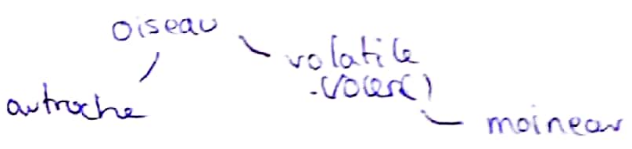
\includegraphics[scale=0.5]{sous-classe-oiseau}
\end{center}
\end{itemize}
%\subsubsection{Classe virtuelle}
%\begin{itemize}
%\item C'est lorsque l'on veut déléguer le traitement
%\item Je veux appeler la méthode de l'objet qui est %en mémoire
%\item Je veux que le traitement appelé soit fait sur la classe concrète/tangible
%\end{itemize}
\subsubsection{Classe abstraite}
\begin{itemize}
\item \textbf{Classe abstraite :} c'est une classe que l'on ne peut pas instancier. C'est donc pour les objets non tangibles.
\item Une classe est abstraite si elle possède au moins une méthode abstraite
\item On peut créer une instance d'une classe abstraite seulement via un pointeur
\item Un pointeur : 
\begin{itemize}
\item c'est une adresse (c'est pas nouveau)
\item c'est aussi maintenant \textbf{un accés à une couverture fonctionnelle} (nouveau)
\end{itemize}
\item Ex : comme la classe mamifères\\
Les objets tangibles seraient chien, chat, homme, etc...
\item Si on crée un pointeur dans le \textit{main()}, on utilise la syntaxe suivante
\begin{lstlisting}
// Dans le main()
Figure* c = new Cercle{0,0,100};
// Instanciation d'un objet de la classe fille Cercle via un pointeur de la classe mere Figure

c->methode1();
c->methode2();
// Utilisation de -> pour utiliser les methodes avec un pointeur
\end{lstlisting}
\item On met le constructeur en protected : le \textit{main()} ne peut pas instancier d'objet de la classe abstraite
\end{itemize}
\subsubsection{Constructeurs et destructeurs}
\begin{itemize}
\item Schéma de pile : on parle de chaînage
\item Par chaînage, les destructeurs des sous-classes sont appelés en premier suivi du destructeur de la classe mère
\item Pour une classe concrète/tangible, le destructeur est public (on peut l'utiliser dans \textit{main()}.
\item Le destructeur de la classe Figure est public sinon il faudrait avoir un desctructeur spécifique pour chaque classe fille : \textbf{destructeur virtuel}
\item Pourquoi le destructeur de la super classe doit être virtuel ?
\begin{itemize}
\item Dans le cas d'une création d'un pointeur de la classe mère pour instancier un objet de la classe fille
\begin{lstlisting}
Figure* r = new Rectangle{...};
\end{lstlisting}
Si on fait un \textit{delete r} qui est appelé ?
\item \textbf{SANS VIRTUAL} : c'est seulement le destructeur de Figure car \textit{r} est un pointeur de Figure\\
\textbf{DÉLÉTION INCOMPLÈTE}
\item \textbf{AVEC VIRUTUAL} : on va déléguer cette destruction au destructeur de la classe tangible (sous-classe)\\
Les destructeurs sont chainés donc pas besoin d'appeler de destructeur dans le destructeur\\
Au final : 1) le destructeur de Rectangle est appelé, 2) Par chaînage le destructeur de Figure est appelé\\
\textbf{DÉLÉTION COMPLÈTE}

\end{itemize}
\end{itemize}
\subsubsection{Pointeur de classe}
\begin{itemize}
\item Pourquoi utiliser un pointeur de Figure pour instancier un Rectangle ou un Cercle?
\begin{itemize}
\item aspect \textbf{Evolutif} : si on rajoute une sous-classe on pourra la manipuler de la même façon \\
Exemple avec les classes Zoo, Animal, Gazelle, Lion
\begin{itemize}
\item La méthode "enfermer()" de Zoo permet d'enfermer \textbf{tous} les animaux donc on utilse la classe animal pour ne pas spécifier quel animal à enfermer
\begin{lstlisting}
zoo::enfermer(Animal& animal);
\end{lstlisting}
\item On veut avoir une liste d'animaux présents dans le zoo + cette liste peut changer
\begin{lstlisting}
// attribut dans Zoo.h
vector<Animal*> animaux;
\end{lstlisting}
\item On peut utiliser un FOR EACH dans les méthodes pour traiter tout le monde
\end{itemize}
\item \textbf{Maintenance}
\item Permet de ne pas spécifier quelle type de donnée on crée
\item Permet d'avoir une fonction unique pour toutes les sous classes en utilisant un pointeur de la classe mère
\begin{lstlisting}
void destroy(Figure* f) // On peut appeler un Rectangle ou un Cercle
\end{lstlisting}
\end{itemize}
\item \textbf{Polymorphisme :} on s'adresse à des gens différents de la même façon\\
Ex: les feux tricolores veulent dire la même chose pour les automobilistes, les cyclistes, les routiers, etc...
\end{itemize}

\subsection{Huitième Partie}
\subsubsection{Méthode virtuelle}
\begin{itemize}
\item Une méthode virtuelle est une fonction pour laquelle tu préviens le compilateur que le comportement risque d'être modifié par une classe dérivée.
\end{itemize}
\subsubsection{Méthode abstraite }
\begin{itemize}
\item \href{https://www.developpez.net/forums/d740612/c-cpp/cpp/debuter/methode-virtuelle-abstraite/}{Developpez : Explications virtuelle/abstraite}
\item Une méthode abstraite est une méthode virtuelle \textit{(virtual)} pure \textit{(=0)}
\begin{lstlisting}
virtual type nomMethode() = 0; // methode abstraite
\end{lstlisting}
\item Une méthode abstraite doit obligatoirement être créée et implémentée dans les classes filles.
\item MAIS une fonction abstraite peut être implémentée dans la classe mêre : elle sera générale pour toutes les sous-classes
\item On fera le chaînage à la main pour appeler la méthode de la classe mère
\end{itemize}
\subsubsection{Override C++11}
\begin{itemize}
\item Aspect \textbf{Robustesse}
\item C'est une sorte de détrompeur
\item \textit{Override} stipule que l'on est entrain de redéfinir une méthode de la classe mère
\item Le compilateur va nous avertir d'une erreur si l'on fait \textit{override} sur une méthode qui n'existe pas dans la classe mère (erreur de nom, type, arguments,...)
\item Le contrat de la méthode doit être spécifiquement le même
\end{itemize}
\subsubsection{Final}
\begin{itemize}
\item Aspect \textbf{Robustesse}
\item Permet de spécifier que l'on ne veut pas implémenter une nouvelle fois une classe, une méthode etc
\item \textit{Final} avec les classes : stipule que la classe dite \textit{Final} ne peut pas avoir de classe fille
\begin{lstlisting}
class A final {...};
class B : public A {...} // Erreur car A final
\end{lstlisting}
\item \textit{Final} avec une méthode d'une classe : stipule qu'on ne peut pas implémenter la même méthode (contrat identique) dans une classe fille
\begin{lstlisting}
class A {
public:
	virtual void f() final;
}
class B : public A{
public:
	void f(); // Erreur car void f() est final
}
\end{lstlisting}
\end{itemize}
\subsubsection{Constructeur hérité}
\begin{itemize}
\item Pour générer tous les constructeurs de la classe mère dans la classe fille MAIS il faut qu'il y ait la même signature (pas de données suplémentaires dans les classes filles)
\item utiliser le mot clefs \textit{using} et générer les constructeurs
\begin{lstlisting}
// Dans la classe fille (avec meme signature)
using classeMere::classeMere; //genere tous les constructeurs
\end{lstlisting}
\end{itemize}
\subsubsection{Résumé}
\begin{center}
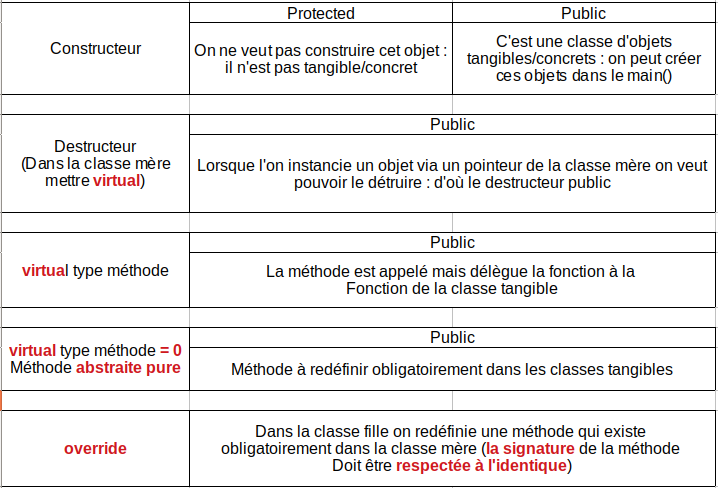
\includegraphics[scale=0.5]{resume}
\end{center}

\subsection{Neuvième Partie}
\subsubsection{STL : Standard Template Library}
\begin{itemize}
\item Les \textbf{conteneurs séquentiels}
\begin{itemize}
\item \textit{Vector} : long en temps pour créer/supprimer un élément MAIS rapide pour accéder aux éléments
\item \textit{List} : facile/rapide pour rajouter/supprimer un élément MAIS lent pour accéder à un élément
\item \textit{Deque} : compromis des deux
\end{itemize}
\item Les \textbf{itérateurs} : \textit{(Polymorphisme)}objet permettant de travailler avec n'importe quel conteneur (se balader dans la collection + pointer les éléments)
\begin{lstlisting}
// v est un vector
begin(v);
end(v); 
// begin et end sont deux iterateurs
\end{lstlisting}
\item Utiliser différentes collections suivant les besoins du projet
\item Dans le projet "Game" on veut faire varier le nombre de joueurs avec la méthode ".enrol"
\begin{lstlisting}
// Dans main()
game.enrol("nomJoueur");
\end{lstlisting}
\begin{itemize}
\item on a interdit l'utilisation du constructeur par copie or c'est quelque chose que les objets de type \textit{vector} utilisent (pour agrandir, diminuer le tableau, sauvegarder les objets dans le tableau, etc...)
\item on utilise donc la collection \textit{list} (est de type liste chaînée donc utilise des pointeurs pour liéer les éléments, pas besoin de constructeur par copie)
\end{itemize}
\end{itemize}
\subsubsection{Bibliographie - Pour la suite}
\begin{itemize}
\item Scott Meyers : "Effective C++"
\item Nicolaï Josuttis : Tout
\item Craig Larman : UML et les Patterns (Design, Analyse)
\end{itemize}

\newpage
\section{Programmation C++}
\subsection{L'héritage}
\begin{itemize}
\item \href{https://openclassrooms.com/fr/courses/1894236-programmez-avec-le-langage-c/1898475-lheritage}{Cours openclassroom : héritage}
\item Déclaration d'une classe héréditaire : 
\begin{lstlisting}
class Classe_fille : public|protected|private Classe_mere1
[, public|protected|private Classe_mere2 [...]]
{
    /* Definition de la classe fille. */
};
\end{lstlisting}
\item les données publiques d'une classe mère deviennent soit publiques, soit protégées, soit privées selon que la classe fille hérite en public, protégé ou en privé.
\item La classe fille possède les attributs et les méthodes de la classe mère. Elle possède en plus de cela ses propres attributs et méthodes
\item Possibilité de surcharger les méthodes de la classe mère dans la classe fille
\item Surcharge du constructeur : on peut appeler le constructeur de la classe mère dans le constructeur de la classe fille.
\newline Pour déclarer un constructeur dans le .h : il doit avoir le même nom que la calsse, et il ne doit rien renvoyer. \textit{maClasse()}
\newline On écrira aussi le constructeur dans le .cpp de la manière suivante : 
\newline \textit{maClasse::maClasse() : blaba, bla, bla \{ \}}
\item Masquage de fonctions de la classe mère. On peut substituer le nom d'une fonction présente dans la classe mère et utiliser sous le même nom une méthode spécifique dans une classe fille. On peut toujours appeler la méthode de la classe mère dans la méthode de la classe fille en spécifiant l'appel à la classe mère grâce au double deux points "nomClasseMere::nomMéthode()".
\item Dérivation de type : on peut substituer un objet de la classe fille à un pointeur ou une référence vers un objet de la classe mère. On peut affecter un élément enfant à un élément parent
\newline Il est possible d'écrire \textit{monPersonnage = monGuerrier} car un guerrier est un personnage. L'inverse n'est pas possible \sout{\textit{monGuerrier = monPersonnage}}
\item La dériation de type est très pratique dans l'appel d'un élément dans une fonction par exemple. Si l'argument à mettre est de la classe \textit{Personnage} il est alors possible de mettre tous les autres classes filles de \textit{Personnage}
\newline \textit{void coupDePoing(Personnage} \& \textit{cible) const;} : \textit{cible} peut être de type \textit{Personnage} ou \textit{Guerrier}
\item Le type \textit{protected} permet aux attributs d'être accessible par les classes filles et inaccessible de l'extérieur
\end{itemize}

\subsection{Polymorphisme}
\begin{itemize}
\item  le polymorphisme est un mécanisme dynamique permettant, par voie d'héritage, de spécialiser dans des classes dérivées les comportements annoncés ou implémentés dans des classes de base, indirectes ou non.
\item \textbf{Résolution statique des liens.} La fonction reçoit un type de data, c'est donc toujours les méthodes de ce type qui sera utilisée. C'est donc le type de la variable qui détermine quelle fonction membre appeler et non sa vraie nature.\\
\textit{Ex pratique : } 
\newline void presenter(Vehicule v)  //Présente le véhicule passé en argument
\newline \{  v.affiche(); \}
\newline La fonction reçoit un véhicule (classe mère) c’est donc les méthodes de véhicule qui sont appelées même si une surcharge de méthode est présente dans la classe fille.
\item \textbf{Réolution dynamique des liens.} Lors de l'exécution le programme utilise la bonne version des méthodes car il sait si l'objet est de type mère ou type fille.
\begin{itemize}
\item utiliser un pointeur ou une référence
\item utiliser des méthodes virtuelles
\end{itemize}
\item Il faut placer un pointeur ou une référence comme argument dans la fonction \textit{void presenter(Vehicule const\& v)}
\item Rajouter \textit{virtual} devant la méthode dans la classe mère (seulement dans le .h) et c’est optionnel dans les classes filles.
\end{itemize}

\subsection{Design Pattern}
\begin{itemize}
\item Ce sont des modèles théoriques adaptables qui résolvent un problème précis.
\item \textbf{Un prototype :} un prototype est une classe dont le but est d'être clonée. 
\item \textbf{Le singleton :} permet de s'assurer qu'il n'existe qu'une unique instance d'une classe donnée. \\
Est une variable globale.
\item \textbf{La fabrique :} classe dont le rôle est de créer d'autres objets.
\item \textbf{Les décorateurs :} sont l'ensemble des classes permettant d'étendre dynamiquement le rôle d'une classe de base.
\end{itemize}

\subsection{Template}
\begin{itemize}
\item Les templates sont des fonctions spéciales qui peuvent être utilisées avec des types génériques. Cela nous permet de créer une fonction template dont l'utilisation n'est pas réstreinte à un seul type de données, sans répéter le code entier pour chaque type.
\begin{lstlisting}
template <class myType>
myType GetMax (myType a, myType b) {
 return (a>b?a:b); }
\end{lstlisting}
\item Pour utiliser les fonctions templates on utilise le schéma suivant :
\begin{lstlisting}
//function_name <type> (parameters);
int x,y;
GetMax <int> (x,y);
\end{lstlisting}
\item Utilisation des templates avec les classes :
\begin{lstlisting}
template <class T>
class mypair {
    T a, b;
  public:
    mypair (T first, T second)
      {a=first; b=second;}
    T getmax ();
};

template <class T> //T for template parameter
T mypair<T>::getmax () //1st T for the type return by the function
//2nd T for requirement to specify the function's template parameter
{
  T retval;
  retval = a>b? a : b;
  return retval;
}
\end{lstlisting}
\end{itemize}

\subsection{Autre}
\begin{itemize}
\item Utilisation de $=$ dans un \textit{if}.
\begin{lstlisting}
int a = 1
int b = 2;
if ((a=b)) {...} //is true
blabla...
int b = 0;
if ((a=b)) {...} //is false
\end{lstlisting}
\item Utilisation de \textit{auto} (C++11) : cet outil permet de spécifier automatiquement le type de la variable en jeu. 
\newline \textit{ex : auto x = 1; auto y = 3.1; auto z = 'a';}
\newline \textit{output : x est int, y est double, z est char}
\item \textit{Lambda} function : \textit{ex : auto allowed = [\&](int x, const std::vector$\langle$int$\rangle$\&vect)\{...\}}
\begin{itemize}
\item a. [=] capture all variables within scope by value
\item b. [\&] capture all variables within scope by reference
\item c. [\& var] capture var by reference
\item d. [\&, var] specify that the default way of capturing is by reference and we want to capture var
\item e. [=, \& var] capture the variables in scope by value by default, but capture var using reference instead.
\end{itemize}
\end{itemize}

\end{document}
